\documentclass{article}
\usepackage{mathtools}
\usepackage{xfrac}
\usepackage{amsfonts}
\usepackage{amsthm}
\usepackage{subfig}
\usepackage{hyperref}
\usepackage{xcolor}

\usepackage{times}
\usepackage{float}

\usepackage[square,numbers]{natbib}
\usepackage[nonatbib]{nips_2018}

\usepackage{bbm}
\usepackage{algorithm, algorithmic}

\newtheorem{theorem}{Theorem}
\newtheorem{lemma}{Lemma}

\allowdisplaybreaks

\renewcommand{\algorithmicrequire}{\textbf{Input:}}
\renewcommand{\algorithmicreturn}{\textbf{Output:}}

% \setlength{\belowcaptionskip}{-15pt}
%  \usepackage[small,compact]{titlesec}
%  \titlespacing{\section}{0pt}{1ex}{0.8ex}
%  \titlespacing{\subsection}{0pt}{0.5ex}{0ex}
%  \titlespacing{\subsubsection}{0pt}{0.2ex}{0ex}
%  \expandafter\def\expandafter\normalsize\expandafter{%
%      \normalsize
%      \setlength\abovedisplayskip{2pt}
%      \setlength\belowdisplayskip{2pt}
%      \setlength\abovedisplayshortskip{0pt}
%      \setlength\belowdisplayshortskip{0pt}
%  }
%  \renewcommand{\baselinestretch}{0.99}

\title{Uncertainty propagation in neural networks for sparse coding}

\author{} % LEAVE BLANK FOR ORIGINAL SUBMISSION.
          % UAI  reviewing is double-blind.

% The author names and affiliations should appear only in the accepted paper.
%
%\author{ {\bf Harry Q.~Bovik\thanks{Footnote for author to give an
%alternate address.}} \\
%Computer Science Dept. \\
%Cranberry University\\
%Pittsburgh, PA 15213 \\
%\And
%{\bf Coauthor}  \\
%Affiliation          \\
%Address \\
%\And
%{\bf Coauthor}   \\
%Affiliation \\
%Address    \\
%(if needed)\\
%}

%\author{ {\bf Danil Kuzin} \\
%\And
%{\bf Olga Isupova}  \\
%\And
%{\bf Lyudmila Mihaylova}   \\
%}

\begin{document}

\maketitle

\begin{abstract}
Despite the recent overwhelming success of deep learning uncertainty estimation is still a challenge for most modern deep learning methods.
The Bayesian learning allows to estimate the uncertainty of predictions in neural networks by imposing the prior distributions on weights, propagating the resulting uncertainty through the layers and computing the posterior distributions of predictions. We propose a novel method of propagating the uncertainty through the soft thresholding nonlinearity. The method expands the area of Bayesian neural networks and enables the soft thresholding nonlinearity to be included in Bayesian deep neural networks for the first time. As an example, we design a Bayesian Learned Iterative Shrinkage-Thresholding network (Bayesian \textsc{lista}). We develop a highly efficient posterior inference algorithm based on probabilistic backpropagation. A series of experiments on sparse coding shows that the proposed framework provides both accurate predictions and sensible estimates of uncertainty in these predictions.
\end{abstract}

\section{Introduction}
The idea of Bayesian learning in neural networks \cite{neal2012bayesian} has recently regained its attention with the development of distributed approximate inference techniques \cite{li2015stochastic, hoffman2013stochastic} and general boost in popularity of deep learning. In addition to algorithms' predictions themselves, Bayesian learning naturally provides the uncertainty estimates of these predictions. These uncertainty estimates are vital, e.g., in spheres that affect people's health, such as self-driving cars or medicine.

In general, when distributions are included in the network, the complexity of Bayesian inference scales exponentially with the number of layers. Nevertheless, recently several techniques have been proposed to handle specific types of neural networks without this exponential growth. For example, feed-forward networks with the rectified linear unit nonlinearity~\cite{hernandez2015probabilistic}, networks with discrete distributions~\cite{soudry2014expectation}, recurrent networks~\cite{mcdermott2017bayesian}.

There are currently two approaches in Bayesian neural networks: explicit distributions of weights can be included in a network \cite{hernandez2015probabilistic, ranganath2015deep}, or dropout can be interpreted as an element introducing uncertainty \cite{gal2016dropout}. We use the former approach and impose prior distributions on the neural network's weights to obtain the posterior distributions of weights and posterior predictive distributions of target variables.

In this paper, we consider the area of sparse coding. The sparse coding problem can be viewed as a linear regression problem with the additional assumption that the majority of the basis representation coefficients should be zeros. This sparsity assumption may be represented as $l1$ penalty~\cite{tibshirani1996regression}, or, in Bayesian interpretation, as a prior that has a sharp peak at zero~\cite{tipping2001sparse}. One of the modern approaches for sparse coding utilises neural networks with the soft thresholding nonlinearity~\cite{gregor2010learning, sprechmann2015learning}. At every layer this nonlinearity shifts current estimates of the target vectors towards zero, which allows to achieve sparsity of the target vectors. Sparse coding is widely used in different applications, such as compressive sensing~\cite{candes2008introduction}, image and video processing~\cite{mairal2014sparse, wang2015deep}, neuroscience~\cite{baillet1997bayesian, jas2017learning}.

In this paper we propose a method to propagate uncertainty through the soft thresholding nonlinearity. At every layer the current distribution of the target vector is represented as a spike and slab distribution \cite{mitchell1988bayesian}, which represents the probabilities of each variable being zero, or Gaussian-distributed. We show that the spike and slab distribution of target vectors can be effectively combined with Gaussian weights of dense layers. The distribution of the target vector propagated through a dense layer and the soft thresholding nonlinearity can then be closely approximated with a distribution from the same family. The proposed method of uncertainty propagation for the soft thresholding nonlinearity allows us to derive the gradients of the logarithms of normalisation constants, which can be used to update a weight distribution. We then develop a highly efficient Bayesian inference algorithm based on the probabilistic backpropagation paradigm while significantly expanding it.

The main contributions of this paper are: (\textit{i}) for the first time we propose a method for uncertainty propagation through the soft thresholding nonlinearity for a Bayesian neural network; (\textit{ii}) we develop an efficient posterior inference algorithm for weights and outputs of neural networks with the soft thresholding nonlinearity; (\textit{iii}) we design a novel Bayesian neural network for sparse coding.

The paper is organised as following: first, we review neural networks for sparse coding in section \ref{sec:nn_sc} and present a novel Bayesian neural network in section \ref{sec:bayesian_lista}. We then describe uncertainty propagation to obtain the spike and slab distribution for an output of a network in section \ref{sec:fprop} and how probabilistic backpropagation is organised to update distributions of weights in section \ref{sec:backpropagation}. After that, we show the experimental results of the algorithm in section \ref{sec:experiments} and finish with discussion and conclusions in section \ref{sec:conclusions}.

\section{Neural networks for sparse coding}
\label{sec:nn_sc}
The neural network approach to sparse coding is based on earlier Iterative Shrinkage and Thresholding Algorithm (\textsc{ista}) \cite{daubechies2004iterative}. It addresses the sparse coding problem as the linear regression problem with $l1$ penalty that promotes sparsity. For the linear regression model with observations $\mathbf{y} \in \mathbb{R}^K$, the design matrix $\mathbf{X} \in \mathbb{R}^{K \times D}$, and the sparse unknown vector of weights $\boldsymbol\beta \in \mathbb{R}^D$, \textsc{ista} minimises the energy function $E(\cdot)$ to find $\boldsymbol\beta$
\begin{equation}
\label{eq:regression_problem}
E(\mathbf{y}, \boldsymbol\beta) = ||\mathbf{X}\boldsymbol\beta - \mathbf{y}||_2^2 + \alpha ||\boldsymbol\beta||_1,
\end{equation}
where $\alpha$ is the parameter that controls the influence of sparse penalty.

At every iteration $l$, \textsc{ista} obtains the new estimate $\widehat{\boldsymbol\beta}_l$ of the target vector $\boldsymbol\beta$ as the linear transformation $\mathbf{b} = \mathbf{W}\mathbf{y} + \mathbf{S}\widehat{\boldsymbol\beta}_{l-1}$ of the input $\mathbf{y}$ with the previous estimate propagated through the soft thresholding function $h_\lambda(\cdot)$
\begin{equation}
h_\lambda(\mathbf{b}) = \text{sgn}(\mathbf{b}) \max(|\mathbf{b}| - \lambda, 0),
\end{equation}
where $\lambda$ is a shrinkage parameter.
In \textsc{ista}, weights of the linear transformation are assumed fixed: $\mathbf{W} = \mathbf{X}^\top / E$, where $E$ is the upper bound of the largest eigenvalue of $\mathbf{X}^\top\mathbf{X}$, and $\mathbf{S} = \mathbf{I}_{D \times D} - \mathbf{W}\mathbf{X}$, where $\mathbf{I}_{D \times D}$ is the identity matrix of size $D$.

The Learned \textsc{ista} (\textsc{lista}) \cite{gregor2010learning} allows to learn the values of matrices $\mathbf{W}$, $\mathbf{S}$ based on a set of pairs $\{\mathbf{Y}, \mathbf{B}\}=\{\mathbf{y}^{(n)}, \boldsymbol\beta^{(n)}\}_{n=1}^N$, where $N$ is the number of these pairs. To achieve this, the \textsc{ista} is limited with the fixed amount of iterations $L$, and interpreted as a recurrent neural network: every iteration of \textsc{ista} corresponds to the layer of \textsc{lista}. A coefficient vector $\boldsymbol\beta$ for an observation~$\mathbf{y}$ is predicted according to Algorithm~\ref{alg:lista}.

\begin{algorithm}[h]
  \caption{\textsc{lista} forward propagation}
  \label{alg:lista}
  \begin{algorithmic}[1]
    \REQUIRE observations $\mathbf{y}$, weights $\mathbf{W}, \mathbf{S}$, number of layers $L$
    \STATE \textit{Initialisation.} Dense layer $\mathbf{b} \gets \mathbf{W}\mathbf{y}$ \label{eq:first_layer}
    \STATE \textit{Initialisation.} Soft thresholding nonlinearity $\widehat{\boldsymbol\beta}_0 \gets h_\lambda(\mathbf{b})$ \label{eq:thr_first}
		\FOR{$l=1$ \TO $L$}
			\STATE Dense layer $\mathbf{c}_l \gets \mathbf{b} + \mathbf{S}\widehat{\boldsymbol\beta}_{l-1}$ \label{eq:l_dense_layer}
			\STATE Soft thresholding nonlinearity $\widehat{\boldsymbol\beta}_{l} \gets h_\lambda(\mathbf{c}_l)$ \label{eq:l_thr}
		\ENDFOR
		\RETURN $\widehat{\boldsymbol\beta} \gets \widehat{\boldsymbol\beta}_{L}$
  \end{algorithmic}
\end{algorithm}

% \begin{align}
% \label{eq:first_layer}
% &\mathbf{b} = \mathbf{W}\mathbf{y}\\
% \label{eq:thr_first}
% &\widehat{\boldsymbol\beta}_0 = h_\lambda(\mathbf{b}) \\
% &\text{for } l=1:L\\
% \label{eq:l_dense_layer}
% 	&\quad \mathbf{c}_l = \mathbf{b} + \mathbf{S}\widehat{\boldsymbol\beta}_{l-1} \\
% \label{eq:l_thr}
% 	&\quad \widehat{\boldsymbol\beta}_{l} = h_\lambda(\mathbf{c}_l) \\
% & \widehat{\boldsymbol\beta} = \widehat{\boldsymbol\beta}_{L}
% \end{align}

In \textsc{lista}, matrices $\mathbf{W}$, $\mathbf{S}$ are the parameters that are initialised as in the \textsc{ista} and then updated with the backpropagation algorithm. Vectors $\mathbf{c}_l$ and $\mathbf{b}$ are auxiliary vectors that describe forward propagation.

\section{Bayesian neural network for sparse coding}
\label{sec:bayesian_lista}
To formulate the Bayesian version of the \textsc{lista} we impose the prior distributions on the unknown weights
\begin{equation}
\label{eq:ws}
p(\mathbf{W}) = \prod_{d=1}^D\prod_{k=1}^K \mathcal{N}(w_{ij} ; 0, \eta^{-1}), \qquad
p(\mathbf{S}) = \prod_{d'=1}^D\prod_{d''=1}^D \mathcal{N}(s_{d'd''} ; 0, \eta^{-1}),
\end{equation}
where $\eta$ is the precision of the Gaussian distribution.

For every layer of the Bayesian \textsc{lista} we assume that $\widehat{\boldsymbol\beta}_{l-1}$ has the spike and slab distribution with spike probability $\boldsymbol\omega$, slab mean $\mathbf{m}$, and slab variance $\mathbf{v}$
\begin{equation}
[\widehat{\boldsymbol\beta}_{l-1}]_d \sim \omega_d \delta_0 + (1 - \omega_d)\mathcal{N}(m_d, v_d),
\end{equation}
where $\delta_0$ is the delta-function that represents a spike, $[\cdot]_d$ denotes the $d$-th component of a vector. In Section \ref{sec:fprop}, we show that the output of the next layer $\widehat{\boldsymbol\beta}_l$ can be approximated with a spike and slab distribution and, therefore, the output of the \textsc{lista} network $\widehat{\boldsymbol\beta}$ has the spike and slab distribution.

To introduce the uncertainty of predictions, we assume that the true $\boldsymbol\beta$ has a Gaussian distribution centered at the output of the \textsc{lista} network with precision $\gamma$. Then the likelihood of $\mathbf{B}$ is defined as
\begin{equation}
\label{eq:likelihood}
p(\mathbf{B}| \mathbf{Y}, \mathbf{W}, \mathbf{S}, \gamma, \lambda) = \prod_{n=1}^N\prod_{d=1}^D\mathcal{N}\left(\beta_d^{(n)}; [\widehat{\boldsymbol\beta}^{(n)}]_d, \gamma^{-1}\right)
\end{equation}
The introduced Gaussian precisions have Gamma prior distributions with parameters~$a^{\cdot}$ and~$b^{\cdot}$
\begin{equation}
\label{eq:gamma_eta}
p(\gamma) = \text{Gam}\left(\gamma; a^{\gamma}, b^{\gamma}\right), \qquad
p(\eta) = \text{Gam}\left(\eta; 	a^{\eta}, b^{\eta}\right)
\end{equation}

The posterior distribution is then
\begin{equation}
\label{eq:posterior}
p(\mathbf{W}, \mathbf{S}, \gamma, \eta | \mathbf{B}, \mathbf{Y}, \lambda) = \frac{p(\mathbf{B} | \mathbf{Y}, \mathbf{W},  \mathbf{S}, \gamma, \lambda) p(\mathbf{W} | \eta )p(\mathbf{S} | \eta) p(\eta) p(\gamma)}{p(\mathbf{B} | \mathbf{Y}, \lambda)}
\end{equation}
The shrinkage parameter $\lambda$ is a hyperparameter of the model.

\section{Uncertainty propagation through soft thresholding}
\label{sec:fprop}
We demonstrate that the output of every \textsc{lista} layer $\widehat{\boldsymbol\beta}_l$ can be approximated with a spike and slab distribution. This leads to the proposed probabilistic backpropagation algorithm that is presented in Section~\ref{sec:backpropagation}.

\subsection{Initialisation}
At step \ref{eq:first_layer} of the \textsc{lista} (Algorithm~\ref{alg:lista}) the matrix $\mathbf{W}$ consists of Gaussian-distributed components $w_{dk} \sim \mathcal{N}(m^w_{dk}, v^w_{dk})$, and $\mathbf{y}$ is a deterministic vector. Since the sum of independent Gaussian-distributed variables is a Gaussian variable~\cite{eisenberg2008sum}, $\mathbf{b}$ is a vector of Gaussian-distributed components $b_d \sim \mathcal{N}(m^b_d, v^b_d)$
\begin{equation}
\label{eq:matrix_vector_product}
m^b_d = \sum_{k=1}^Ky_k m^w_{dk}, \qquad
v^b_d = \sum_{k=1}^Ky_k^2v^w_{dk}.
\end{equation}

At step~\ref{eq:thr_first} of the \textsc{lista} (Algorithm~\ref{alg:lista}) the Gaussian vector $\mathbf{b}$ is taken as an input of the soft thresholding function.

When a Gaussian random variable $x \sim \mathcal{N}(x; m, v)$ is propagated through the soft thresholding function $x^* = h_{\lambda}(x)$, the probability mass of the resulting random variable $x^*$ is split into two parts. The values of $x$ from the interval $[-\lambda, \lambda]$ are converted to~$0$ by the soft thresholding operator. Therefore, the probability mass of the original distribution that lies in $[-\lambda, \lambda]$ is squeezed into the probability of $x^*$ being zero. The values of $x$ from outside of the $[-\lambda, \lambda]$ interval are shifted towards~$0$. The distribution of $x^* \neq 0$ then represents the tails of the original Gaussian distribution.

\begin{lemma}[Propagation of a Gaussian variable through soft thresholding]
\label{thm:soft_thresholding}
The distribution of $x^*$ can be parametrised by the probability of being zero, $\omega^*$, the mean $m^*$ and the variance $v^*$ of the truncated Gaussian distribution.
\end{lemma}

The proof of Lemma~\ref{thm:soft_thresholding} and expressions for $\omega^*$, $m^*$ and $v^*$ are given in the supplementary materials. Based on the results of Lemma~\ref{thm:soft_thresholding}, we approximate the distribution of $\widehat{\boldsymbol\beta}_0$ at step~\ref{eq:thr_first} with a spike and slab distribution with parameters derived in the lemma: the spike probability $\omega$ is equal to $\omega^*$, the slab mean $m$ and variance $v$ are set to the corresponding parameters of the truncated Gaussian $m^*$ and $v^*$. The quality of this approximation is discussed in the supplementary materials.

\subsection{Main layers}
At step \ref{eq:l_dense_layer} of the \textsc{lista} (Algorithm~\ref{alg:lista}) the vector $\mathbf{b}$ and matrix $\mathbf{S}$ consist of Gaussian components and $\widehat{\boldsymbol\beta}_{l-1}$ is a vector of the spike and slab random variables. In order to determine the distribution of the output $\mathbf{c}_l$ we first formulate two lemmas.

\begin{lemma}[Moments of a spike and slab distribution]
\label{thm:moments_spsl}
Let a random variable $\xi$ have a spike and slab distribution with the probability of spike $\omega$, the slab mean $m$ and slab variance $v$. Then its moments are
\begin{equation}
\mathbb{E}\xi = (1-\omega)m, \qquad \operatorname{Var}\xi = (1-\omega)(v + \omega m^2)
\end{equation}
\end{lemma}

\begin{lemma}[Product of a Gaussian matrix and a spike and slab vector]
  \label{thm:matrix_vector}
Let $\mathbf{S} \in \mathbb{R}^{D \times D}$ be a matrix of independent Gaussian-distributed random variables: $s_{d'd''} \sim \mathcal{N}(m^s_{d'd''}, v^s_{d'd''})$, and $\widehat{\boldsymbol\beta }\in \mathbb{R}^D$ be a vector with spike-and-slab-distributed variables: $\widehat{\beta}_d \sim \omega_d \delta_0 + (1 - \omega_d)\mathcal{N}(m_d, v_d)$. The components of the matrix $\mathbf{S}$ and the vector $\widehat{\boldsymbol\beta}$ are mutually independent. Let $\mathbf{e} \in \mathbb{R}^{D}$ denote the product $\mathbf{S} \widehat{\boldsymbol\beta}$. Then the marginal mean and variance of the elements $e_d$ of the vector $\mathbf{e}$ are:
\begin{subequations}
\begin{align}
 \mathbb{E}e_d &= \sum_{d'=1}^D m^s_{dd'}(1-\omega_{d'})m_{d'}, \\
 \begin{split}
 \operatorname{Var}e_d &= \sum_{d'=1}^D [(m^s_{dd'})^2(1-\omega_{d'})^2v_{d'} + (1-\omega_{d'})^2(m_{d'})^2v^s_{dd'} + v^s_{dd'}(1-\omega_{d'})^2v_{d'}].
 \end{split}
 \end{align}
\end{subequations}
 \end{lemma}

The proofs of Lemmas~\ref{thm:moments_spsl} and~\ref{thm:matrix_vector} are given in the supplementary materials.

Let $\mathbf{e}_l$ denote the product $\mathbf{S}\widehat{\boldsymbol\beta}_{l-1}$ at step \ref{eq:l_dense_layer} of the Bayesian \textsc{lista}. We assume that $\mathbf{S}$ and $\widehat{\boldsymbol\beta}_{l-1}$ are mutually independent. Then according to the Central Limit Theorem $[ \mathbf{e}_l ]_d$ can be approximated as a Gaussian-distributed variable when $D$ is sufficiently large. The parameters of the of the approximating Gaussian distribution are set to the marginal mean and variance given in Lemma~\ref{thm:matrix_vector}. The supplementary materials provide a discussion of the quality of this approximation.

The output $\mathbf{c}_l$ at step \ref{eq:l_dense_layer} is then represented as a sum of two Gaussian-distributed vectors: $\mathbf{b}$ and~$\mathbf{e}_l$, i.e. it is a Gaussian-distributed vector with components $c_{d} \sim \mathcal{N}(m^c_{d}, v^c_{d})$
\begin{equation}
\label{eq:sum_vectors}
m^c_{d} = m^b_{d} + m^e_{d}, \qquad
v^c_{d} = v^b_{d} + v^e_{d}.
\end{equation}


Then $\widehat{\boldsymbol\beta}_{l}$ at step \ref{eq:l_thr} of the Bayesian \textsc{lista} (Algorithm~\ref{alg:lista}) is the result of soft thresholding of a Gaussian variable, which is approximated with the spike and slab distribution,  similar to step \ref{eq:thr_first}.

\subsection{Bayesian \textsc{lista} forward propagation}
We have covered all steps of the Bayesian \textsc{lista} and derived distributions for outputs of these steps. Now we can formulate the main result of this section that describes how the proposed uncertainty propagation scheme works.

\begin{enumerate}
	\item $\mathbf{b} = \mathbf{W}\mathbf{y}$ is the Gaussian distribution with parameters computed according to (\ref{eq:matrix_vector_product});
	\item $\widehat{\boldsymbol\beta}_{0} = h_\lambda(\mathbf{b})$ is approximated with the spike and slab distribution, which parameters are computed according to Lemma \ref{thm:soft_thresholding}.
	\item $\mathbf{e}_l = \mathbf{S}\widehat{\boldsymbol\beta}_{l-1}$ is approximated with the Gaussian distribution, which parameters are computed according to Lemma \ref{thm:matrix_vector};
	\item $\mathbf{c}_l = \mathbf{b} + \mathbf{e}_l$ is the Gaussian distribution with parameters computed according to (\ref{eq:sum_vectors});
	\item $\widehat{\boldsymbol\beta}_{l} = h_\lambda(\mathbf{c}_l)$ is approximated with the spike and slab distribution, which parameters are computed according to Lemma \ref{thm:soft_thresholding}.
\end{enumerate}




%\subfloat[\textsc{nmse} on validation]{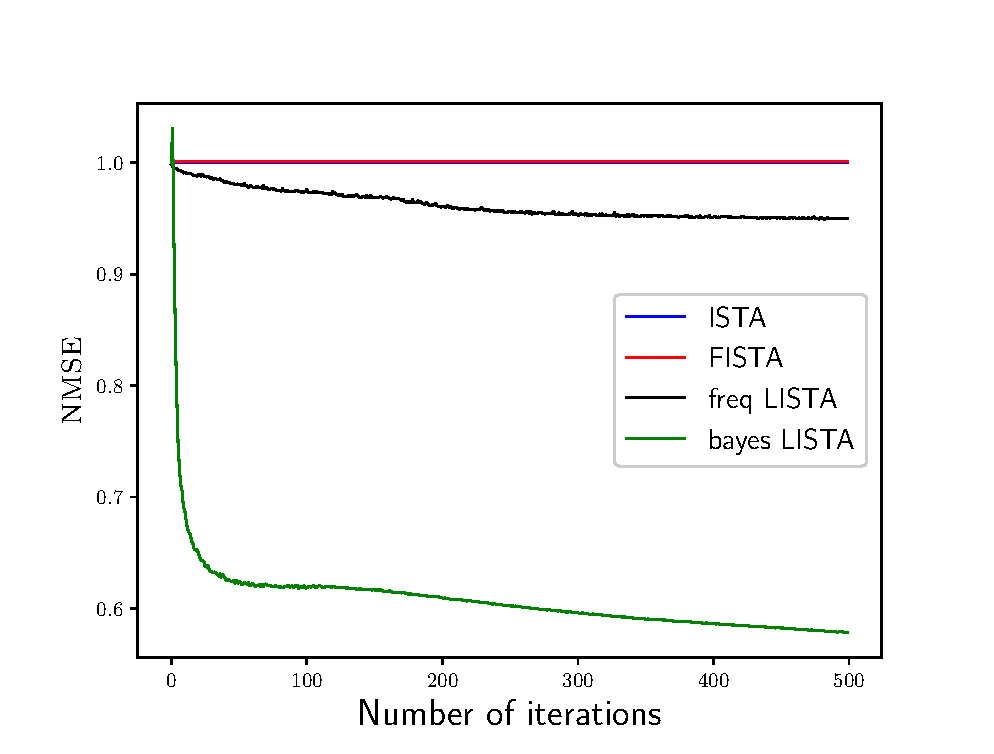
\includegraphics[width=0.5\columnwidth]{graphics/mnist/100_non_normalised_nmse_valid}}

%\begin{figure}[t]
%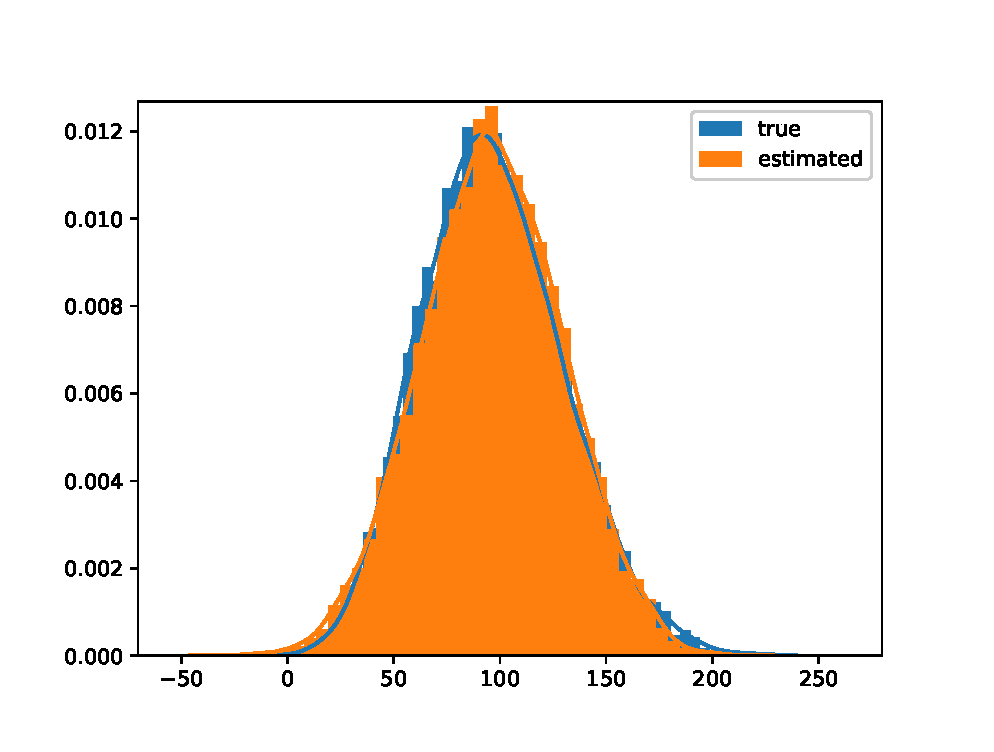
\includegraphics[width=\columnwidth]{d_testing}
%\caption{Approximation of product of Gaussians.}
%\label{fig:d_testing}
%\end{figure}
%
%\begin{figure}[t]
%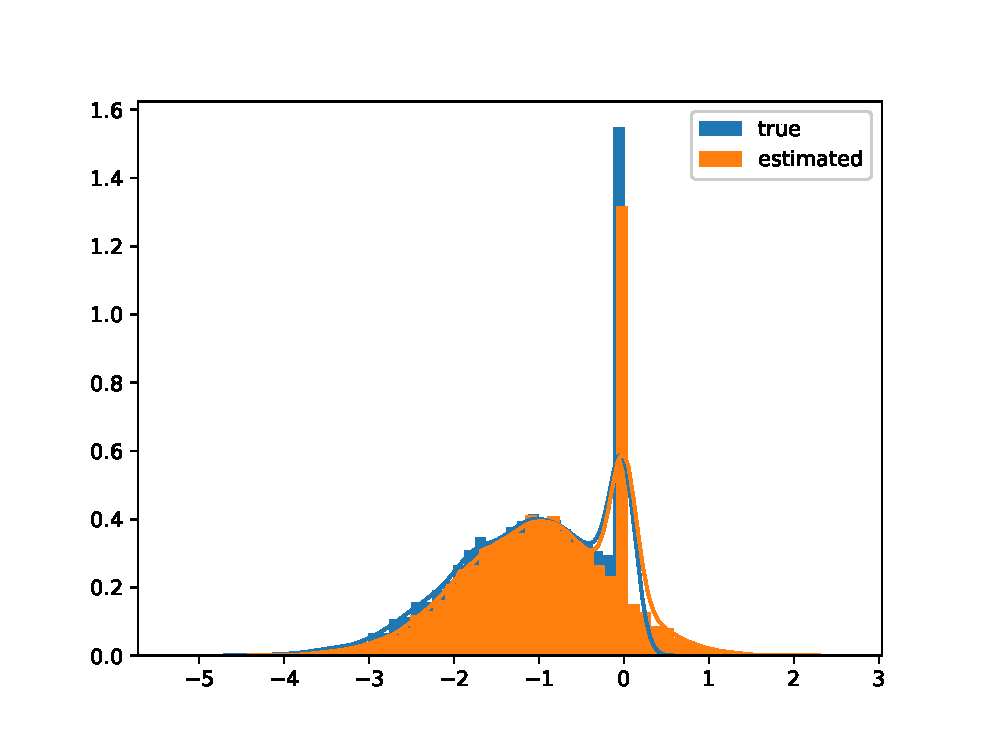
\includegraphics[width=\columnwidth]{z_new_testing}
%\caption{Approximation of propagation through soft thresholding}
%\label{fig:z_new_testing}
%\end{figure}


\section{Backpropagation}
\label{sec:backpropagation}

The exact intractable posterior (\ref{eq:posterior}) is approximated with a factorised distribution
\begin{align}
\label{eq:approximating_dsitribution}
\begin{split}
q(\mathbf{W}, \mathbf{S}, \gamma, \eta) &= \prod_{d=1}^D\prod_{k=1}^K \mathcal{N}(w_{dk} ; m^w_{dk}, v^w_{dk}) \prod_{d'=1}^D\prod_{d''=1}^D \mathcal{N}(s_{d'd''} ; m^s_{d'd''}, v^s_{d'd''}) \\
&\times \text{Gam}(\gamma; a^\gamma, b^\gamma) \text{Gam}(\eta; a^\eta, b^\eta)
\end{split}
\end{align}

For Bayesian inference we expand the probabilistic backpropagation algorithm~\cite{hernandez2015probabilistic} for updating parameters of distributions. They are updated with assumed density filtering (ADF) and expectation propagation (EP) algorithms based on the derivatives of the logarithm of a normalisation constant. ADF iteratively incorporates factors from the true posterior $p$ in (\ref{eq:posterior}) into the factorised approximating distribution $q$ in (\ref{eq:approximating_dsitribution}), whereas EP iteratively replaces factors in $q$ by factors from $p$.

When a factor from $p$ is incorporated into $q$, $q$ as a function of weights $\mathbf{W}$ and $\mathbf{S}$ has the form
\begin{equation}
q(a) = Z^{-1}f(a)\mathcal{N}(a; m, v)
\end{equation}
where $Z$ is the normalisation constant and $f(a)$ is an arbitrary function, $a \in \{w_{dk}, s_{d'd''}\}$.

According to \cite{minka2001thesis}, new parameters of the Gaussian distribution for $a$ can be computed as
\begin{equation}
\label{eq:param_update}
m^{\text{new}} = m + v \frac{\partial \log Z}{\partial m}, \qquad
v^{\text{new}} = v - v^2\left[ \left(\frac{\partial \log Z}{\partial m}\right)^2 - 2 \frac{\partial \log Z}{\partial v}\right]
\end{equation}

Then to find new values of $\mathbf{W}$ and $\mathbf{S}$ we need to compute derivatives of the logarithm of $Z$ when the factor of the true posterior $p$ is incorporated in $q$.

With the likelihood factors~(\ref{eq:likelihood}) of the true posterior we employ the ADF approach and iteratively incorporate them into the approximating distribution $q$. The normalisation constant of the approximating distribution $q$ with the likelihood term for the data point $n$ incorporated can be computed as follows (to simplify notation the superscript $(n)$ is omitted)
\begin{equation}
Z  = \int \prod_{d=1}^{D} \mathcal{N}(\beta_d ; \widehat{\boldsymbol\beta}, \gamma^{-1}) q(\mathbf{W}, \mathbf{S}, \gamma, \eta) \mathrm{d}\mathbf{W} \mathrm{d}\mathbf{S} \mathrm{d}\gamma \mathrm{d}\eta
\end{equation}
Assuming the spike and slab distribution for $\widehat{\boldsymbol\beta}$, the normalisation constant can be approximated as \footnote{Full derivation of the normalisation constant is given in supplementary materials.}
\begin{equation}
\label{eq:Z}
Z \approx \prod_{d=1}^D \left[\omega^{\widehat{\boldsymbol\beta}}_d  \mathcal{T}\left(\beta_d ; 0, \beta^\gamma / \alpha^\gamma, 2\alpha^\gamma\right) + \vphantom{m^{\widehat{\boldsymbol\beta}}_d} \left(1 - \omega^{\widehat{\boldsymbol\beta}}_d\right)\mathcal{N}\left(\beta_d ; m^{\widehat{\boldsymbol\beta}}_d,  \beta^\gamma / (\alpha^\gamma - 1) + v^{\widehat{\boldsymbol\beta}}_d\right)\right],
\end{equation}
where $\{\omega^{\widehat{\boldsymbol\beta}}_d, m^{\widehat{\boldsymbol\beta}}_d, v^{\widehat{\boldsymbol\beta}}_d\}$ are the parameters of the spike and slab distribution for $[\widehat{\boldsymbol\beta}]_d$. Parameters of the approximating posterior distribution $q$ are then updated with the derivatives of this normalisation constant according to (\ref{eq:param_update}).

Prior factors from $p$ (\ref{eq:ws}), (\ref{eq:gamma_eta}) are incorporated into $q$ with the EP algorithm~\cite{hernandez2015probabilistic}, i.e. they replace the corresponding approximating factors from $q$ and then $q$ is updated to minimise the KL divergence.

\section{Experiments}
\label{sec:experiments}
The proposed Bayesian \textsc{lista} is evaluated in the context of the sparse coding problem with an overcomplete dictionary, where the number of measurements $K$ is much smaller than the dimensionality of the vector $\boldsymbol\beta$.

We compare the proposed Bayesian \textsc{lista} with the classical \textsc{lista}~\cite{gregor2010learning} in terms of the predictive accuracy. As baselines we also use the \textsc{ista} \cite{daubechies2004iterative} and Fast \textsc{ista} (\textsc{fista}) \cite{beck2009fast}. The \textsc{fista} adds the momentum to the \textsc{ista} and improves its convergence speed. We set the number of iterations in these algorithms and the number of layers in the Bayesian and classical \textsc{lista} networks to $L$. To measure the performance of the algorithms the normalised mean square error (\textsc{nmse}) and F measure are used\footnote{\textsc{nmse} and F measure are defined in supplementary materials.}. We demonstrate the performance on small datasets to highlight that the proposed algorithm can infer accurate predictions when the dataset size is not sufficient for the \textsc{lista} to learn.

\begin{figure}[t!]
\centering
%\subfloat[\textsc{nmse} on train]{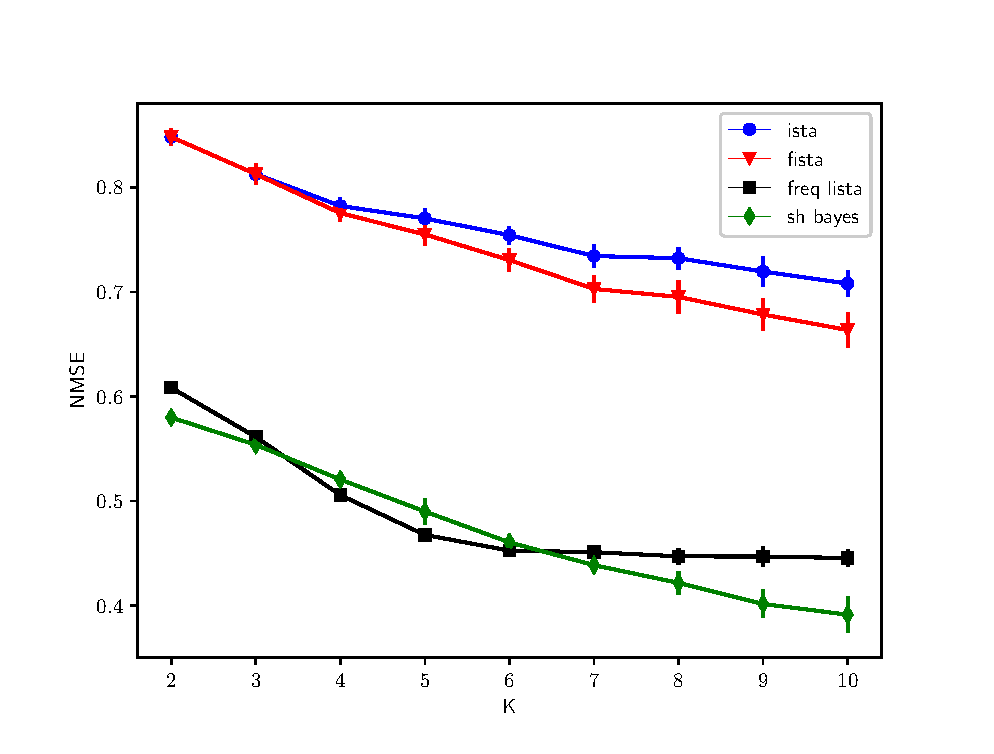
\includegraphics[width=0.5\columnwidth]{graphics/synthetic_number_of_layers/nmse_train}}
%~
\subfloat[\textsc{nmse} for different $L$]{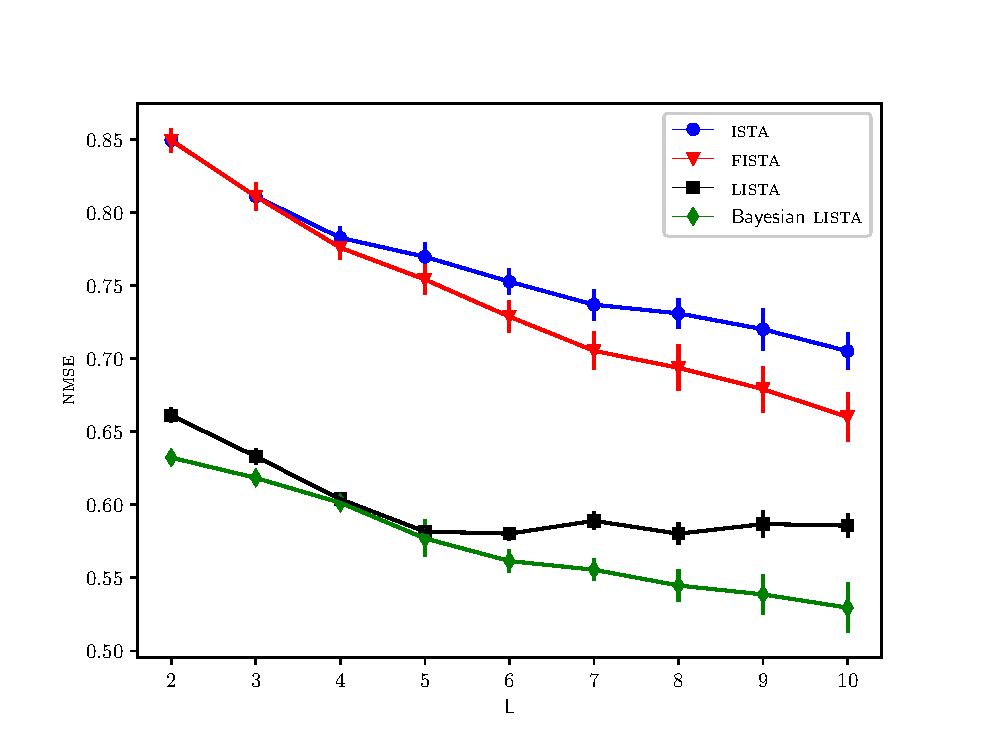
\includegraphics[width=0.4\columnwidth]{graphics/synthetic_number_of_layers/nmse_validation}
\label{fig:nmse_n_layers_synthetic}}
%\subfloat[F measure on train]{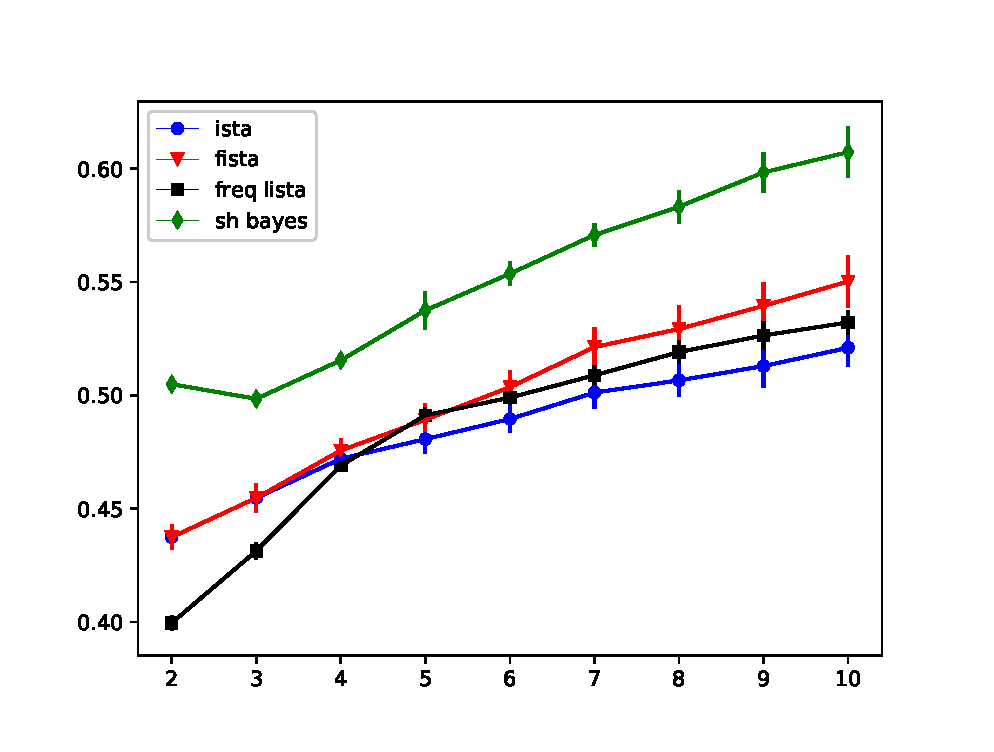
\includegraphics[width=0.5\columnwidth]{graphics/synthetic_number_of_layers/f_measure_train}}
%~
\subfloat[F measure for different $L$]{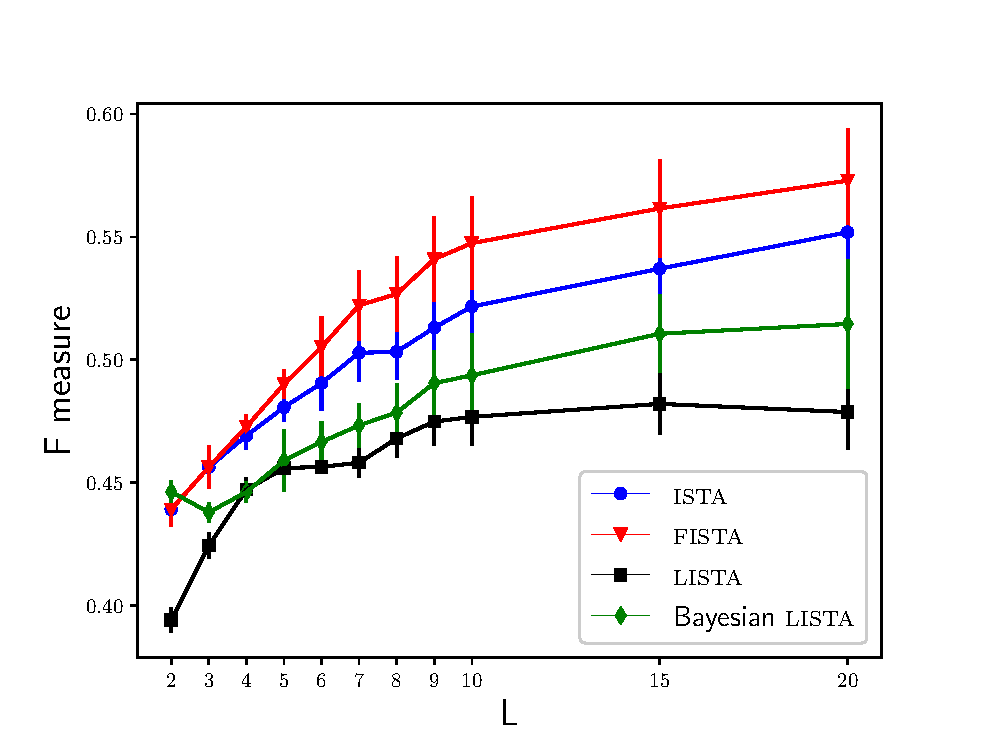
\includegraphics[width=0.4\columnwidth]{graphics/synthetic_number_of_layers/f_measure_validation}
\label{fig:f_meas_n_layers_synthetic}}\\[-13pt]
\subfloat[\textsc{nmse} for different $K$]{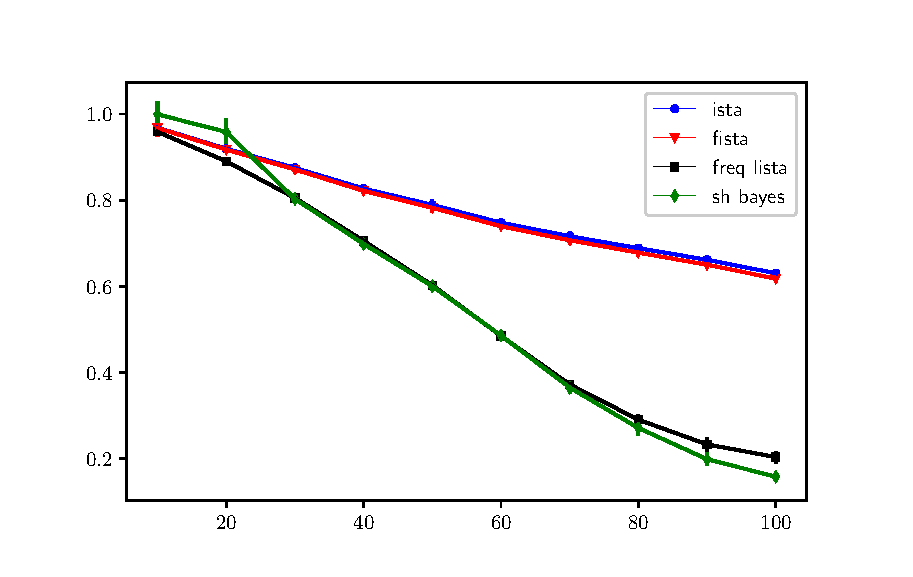
\includegraphics[width=0.4\columnwidth]{graphics/synthetic_undersampling/nmse_validation}
\label{fig:nmse_undersampling_synthetic}}
%\subfloat[F measure on train]{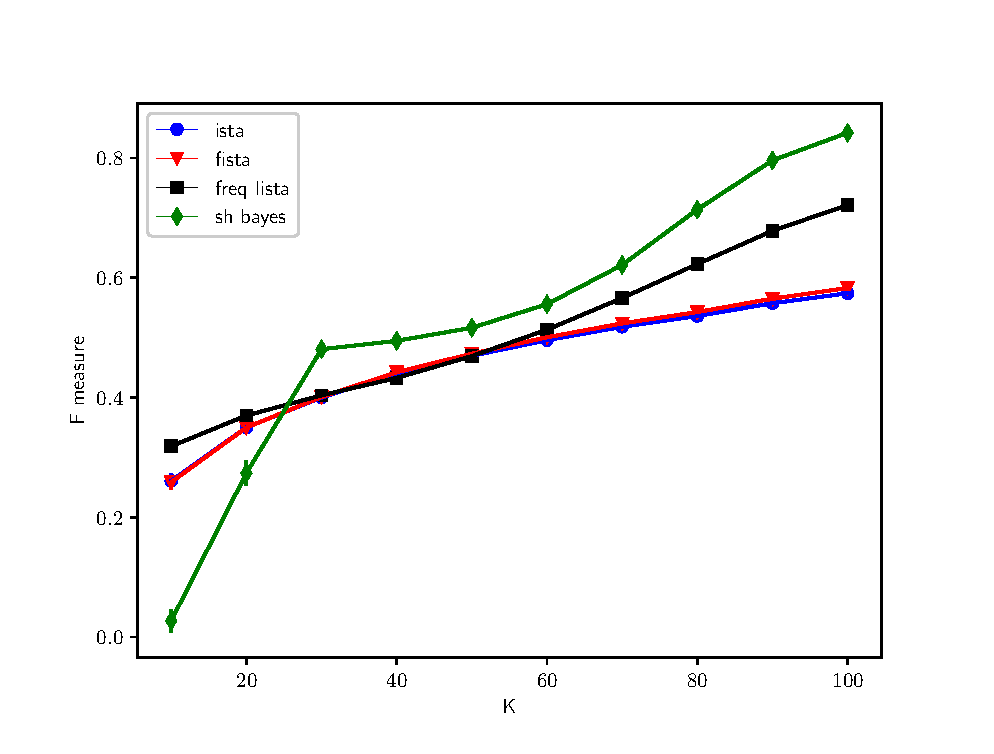
\includegraphics[width=0.5\columnwidth]{graphics/synthetic_undersampling/f_measure_train}}
%~
\subfloat[F measure for different $K$]{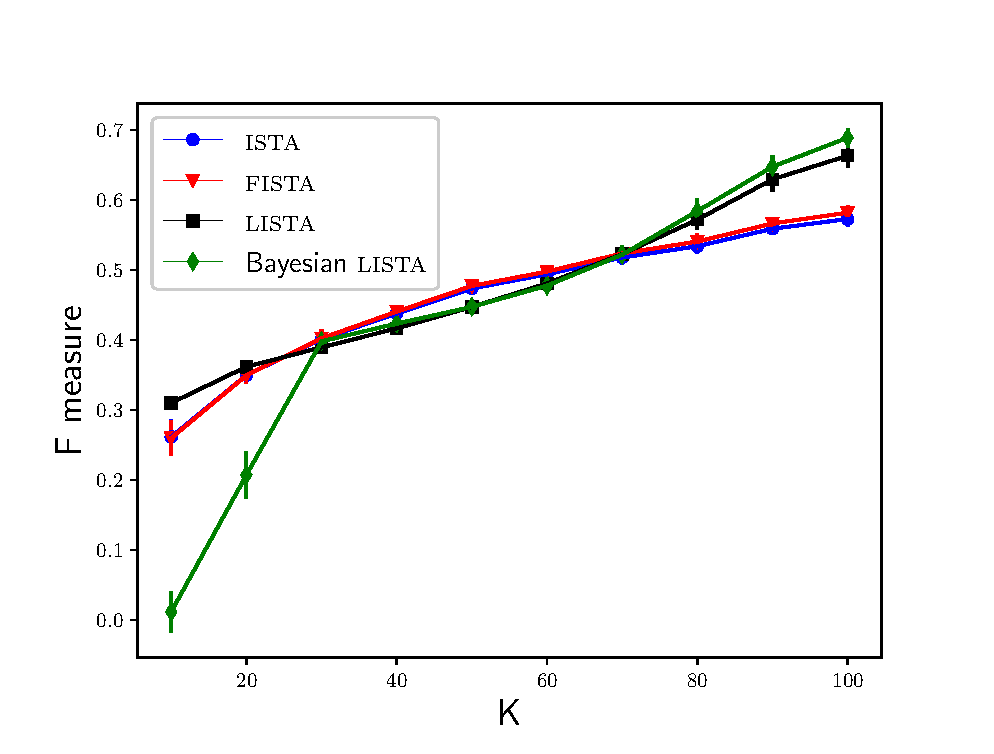
\includegraphics[width=0.4\columnwidth]{graphics/synthetic_undersampling/f_measure_validation}
\label{fig:f_meas_undesampling_synthetic}}
\caption{Predictive accuracy on the synthetic data: the top row for different numbers of layers (for neural networks) or iterations (for baselines),  the bottom row for different sizes of observations}
\label{fig:number_of_layers_synthetic}
\end{figure}

\subsection{Predictive performance on synthetic data}
First, the predictive performance of the proposed Bayesian \textsc{lista} is analysed on synthetic data. We generate $N_\text{train}=1000$ and $N_{\text{test}} = 100$ sparse coefficient vectors $\boldsymbol\beta^{(n)}$ of size $D = 100$  from the spike and slab distribution with the truncated slab: each component $\beta^{(n)}_{d}$ is zero with probability $0.8$ or is sampled from the standard Gaussian distribution without interval $(-0.1, 0.1)$ with probability $0.2$. To simulate sparse observations, we generate the random Gaussian design matrix $\mathbf{X} \in \mathbb{R}^{K \times D}$.  The observations are generated according to (\ref{eq:regression_problem}) with the zero-mean Gaussian noise with the standard deviation $0.5$. The shrinkage parameter is set to~$\lambda = 0.1$. We train the algorithms using the training data of size $N_\text{train}$ and measure performance on the test data of size $N_{\text{test}}$.

In Figures \ref{fig:nmse_n_layers_synthetic} and \ref{fig:f_meas_n_layers_synthetic} predictive performance for different number of layers $L$ is presented. The observation size is set to $K=50$. The Bayesian \textsc{lista} outperforms the \textsc{lista} in terms of both measures. Although the baseline \textsc{ista} and \textsc{fista} show better performance in terms of F measure, the Bayesian \textsc{lista} has the lowest \textsc{nmse}.

Figures~\ref{fig:nmse_undersampling_synthetic} and~\ref{fig:f_meas_undesampling_synthetic} give the results of predictive performance for different observation sizes $K$. The number of layers is set as $L=4$. In the previous experiment the Bayesian and classical \textsc{lista} show similar results with this number of layers. The results of Figures~\ref{fig:nmse_undersampling_synthetic} and~\ref{fig:f_meas_undesampling_synthetic} confirm this competitive behaviour between two \textsc{lista} networks. Baselines show similar results in terms of F measure and underperform in terms of \textsc{nmse}. Overall, the experiments on the synthetic data demonstrate that the Bayesian \textsc{lista} provides competitive results in terms of predictive accuracy.

%We compare two versions of the proposed Bayesian LISTA: with shared weight matrices and with individual matrices at each layer --- and LISTA.

%The NMSE is presented in figure \ref{fig:validation_synthetic}.
%\begin{figure}[t]
%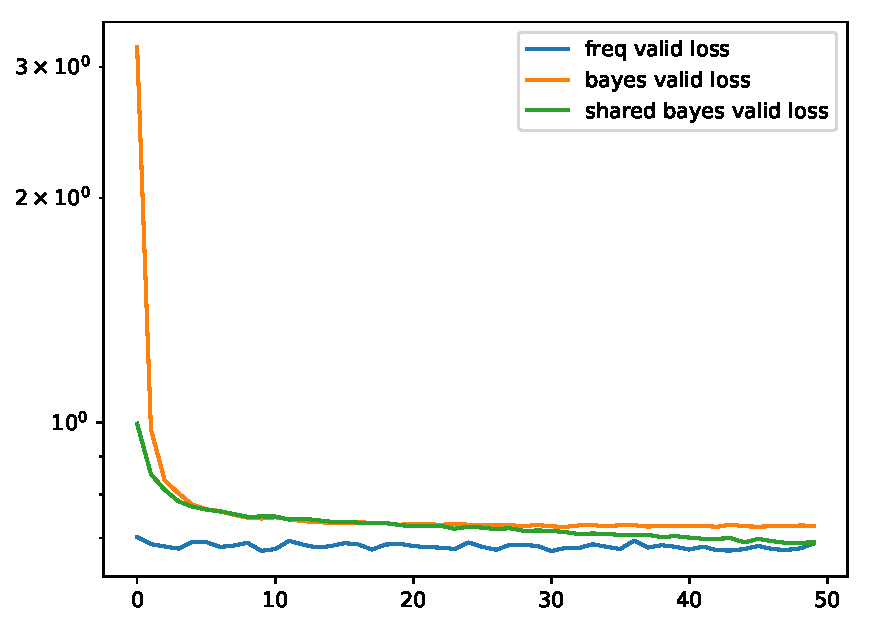
\includegraphics[width=\columnwidth]{loss_synthetic}
%\caption{Validation NMSE on synthetic data}
%\label{fig:validation_synthetic}
%\end{figure}

\subsection{Predictive performance on \textsc{mnist} data}
In this experiment we evaluate the proposed Bayesian \textsc{lista} in terms of predictive performance on the \textsc{mnist} dataset \cite{lecun1998gradient}. The dataset contains images of handwritten digits of size $28 \times 28 = 784$. The design matrix $\mathbf{X}$ is generated as standard random Gaussian. The resulting size of $\mathbf{X}$ is $K \times 784$. Then we generate observations as $\mathbf{y} = \mathbf{X}\boldsymbol\beta$, where $\boldsymbol\beta \in \mathbb{R}^{784}$ are flattened images. We use $100$ images for training and $100$ for test. The shrinkage parameter $\lambda$ is fixed as $0.1$.

Figure \ref{fig:mnist} presents quality results on the validation set with observation sizes $100$ and $250$. The experiment with $K=100$ presents severe conditions for the algorithms: the very limited size of the training dataset combined with the small dimensionality of observations. The Bayesian \textsc{lista} is able to learn under these conditions, outperforming the \textsc{lista} that demonstrates poor results. Under better conditions of the second experiment with $K=250$, both \textsc{lista} networks converge to the similar results. However, the Bayesian \textsc{lista} demonstrates remarkably better convergence rate. Both baselines are unable to perform well in these experiments. Further results on investigation of the predicted posterior and clock time comparison are given in the supplementary materials.

\begin{figure}[h]
\centering
%\subfloat[\textsc{nmse} on train]{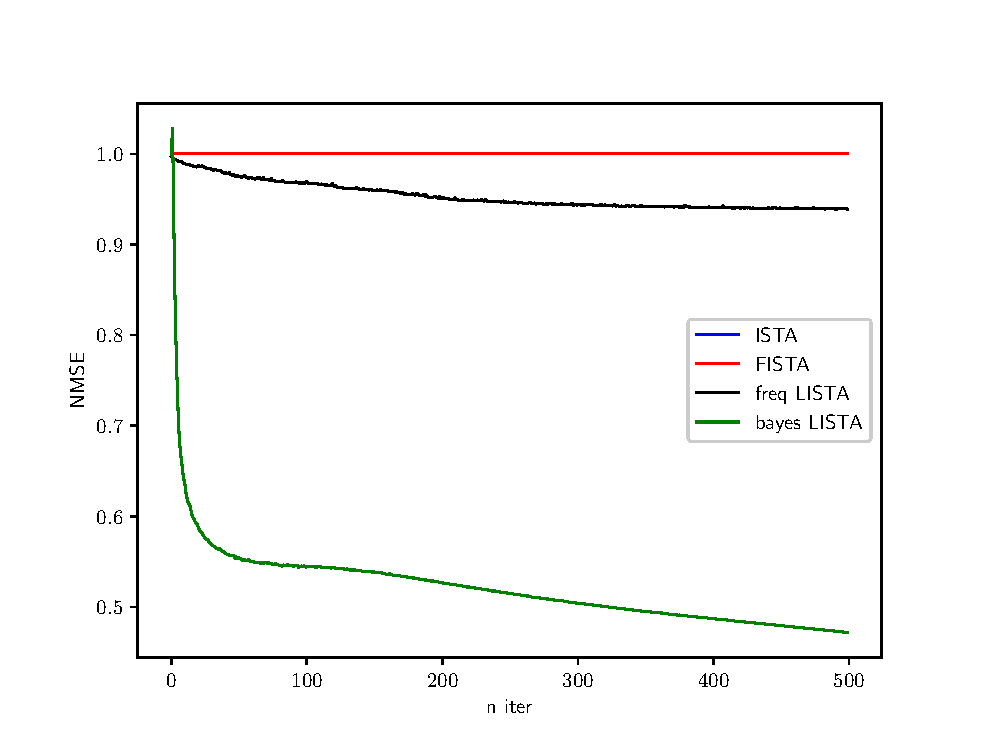
\includegraphics[width=0.5\columnwidth]{graphics/mnist/100_normalised_nmse_train}}
%~
\subfloat[\textsc{nmse} for $K = 100$]{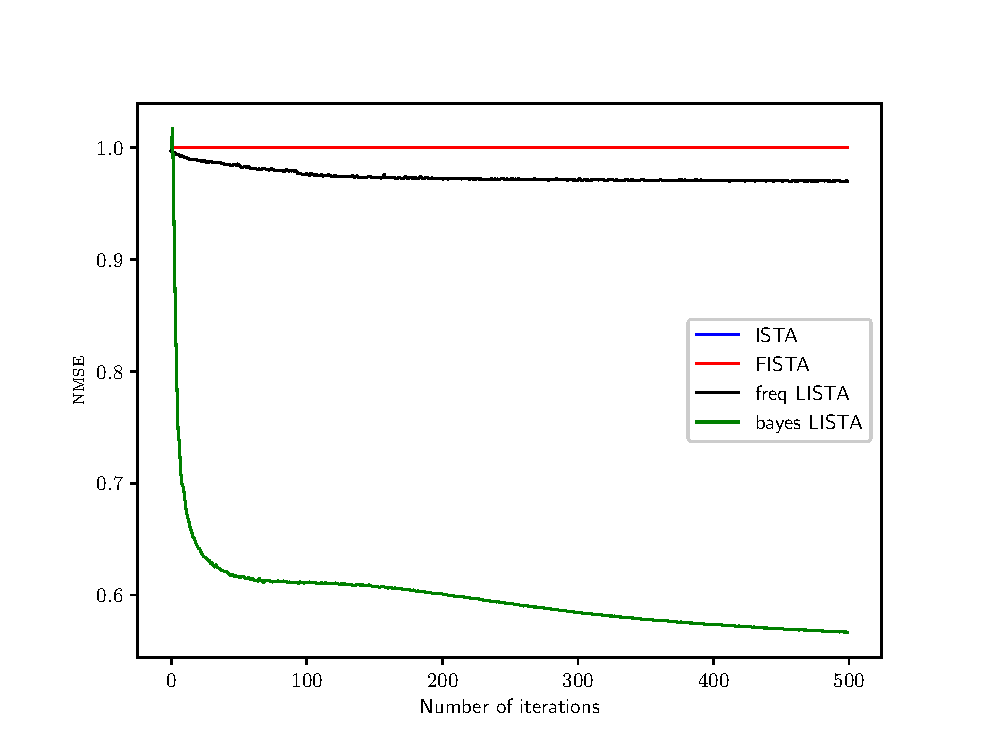
\includegraphics[width=0.4\columnwidth]{graphics/mnist/100_nmse_valid}}
%\subfloat[F measure on train]{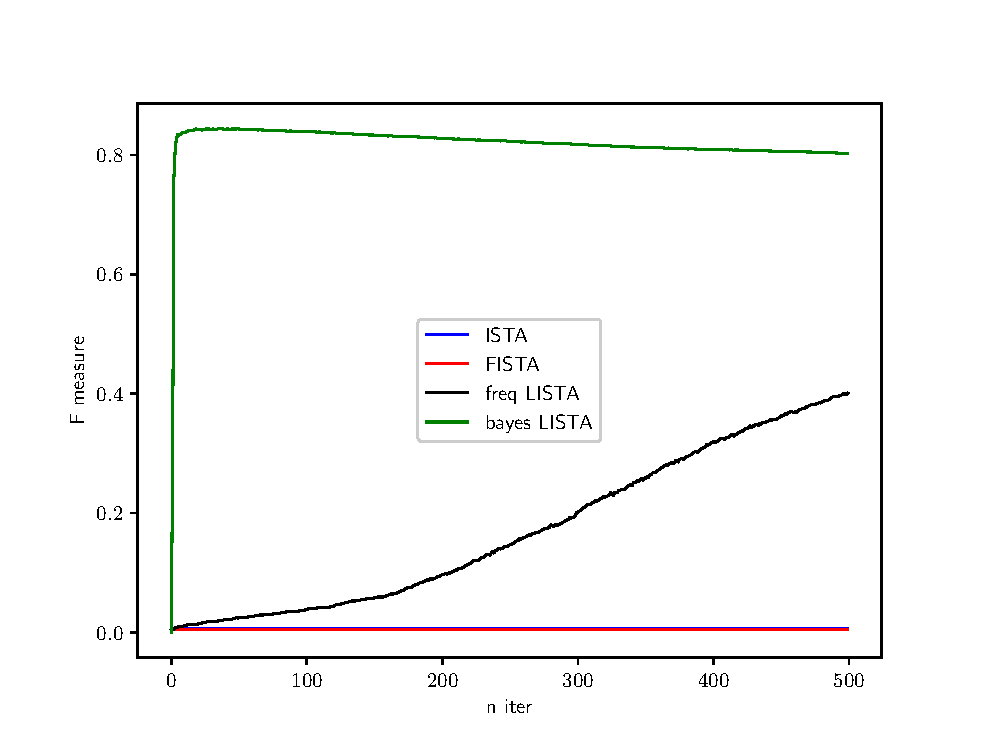
\includegraphics[width=0.5\columnwidth]{graphics/mnist/100_normalised_f_measure_train}}
%~
\subfloat[F measure for $K = 100$]{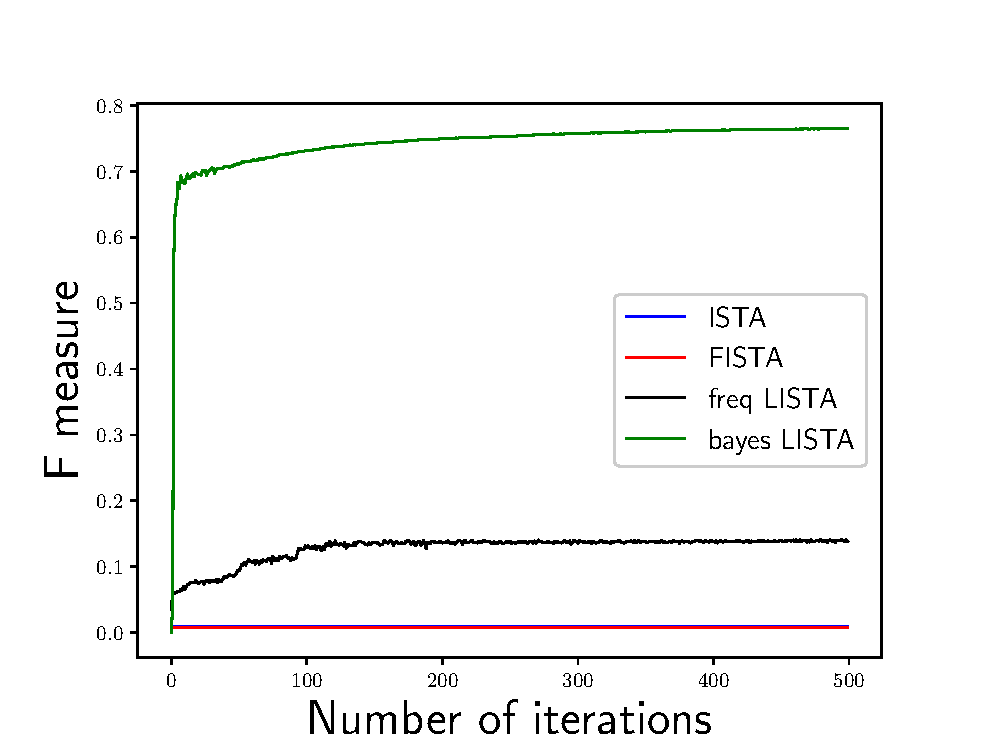
\includegraphics[width=0.4\columnwidth]{graphics/mnist/100_f_measure_valid}}\\[-13pt]
\subfloat[\textsc{nmse} for $K = 250$]{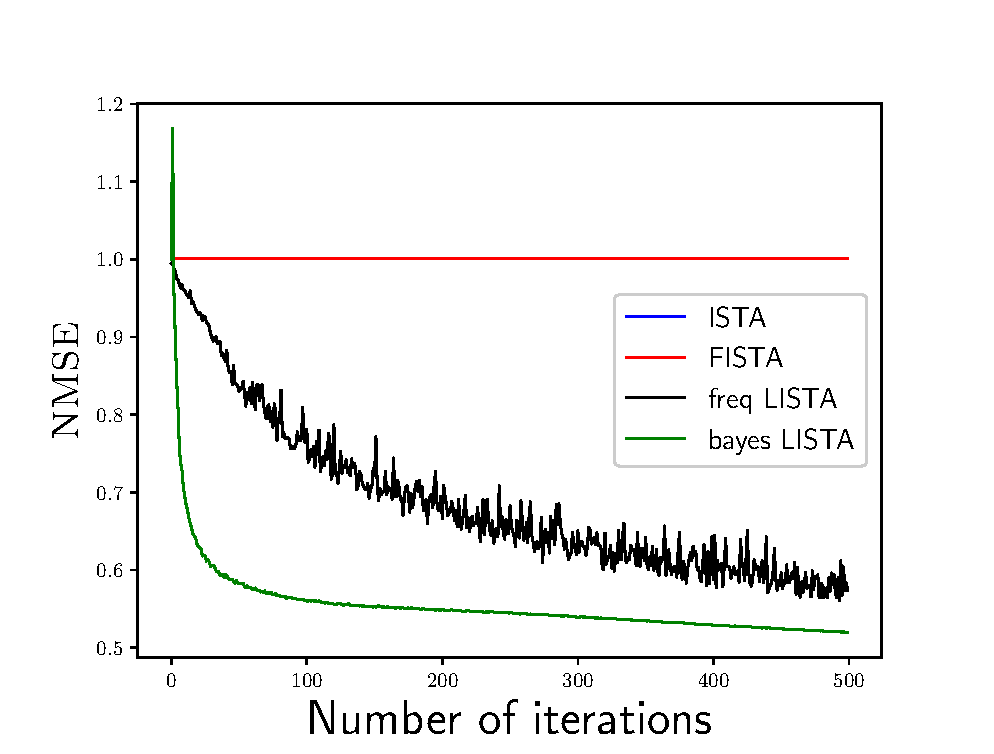
\includegraphics[width=0.4\columnwidth]{graphics/mnist/250_nmse_valid}}
%\subfloat[F measure on train]{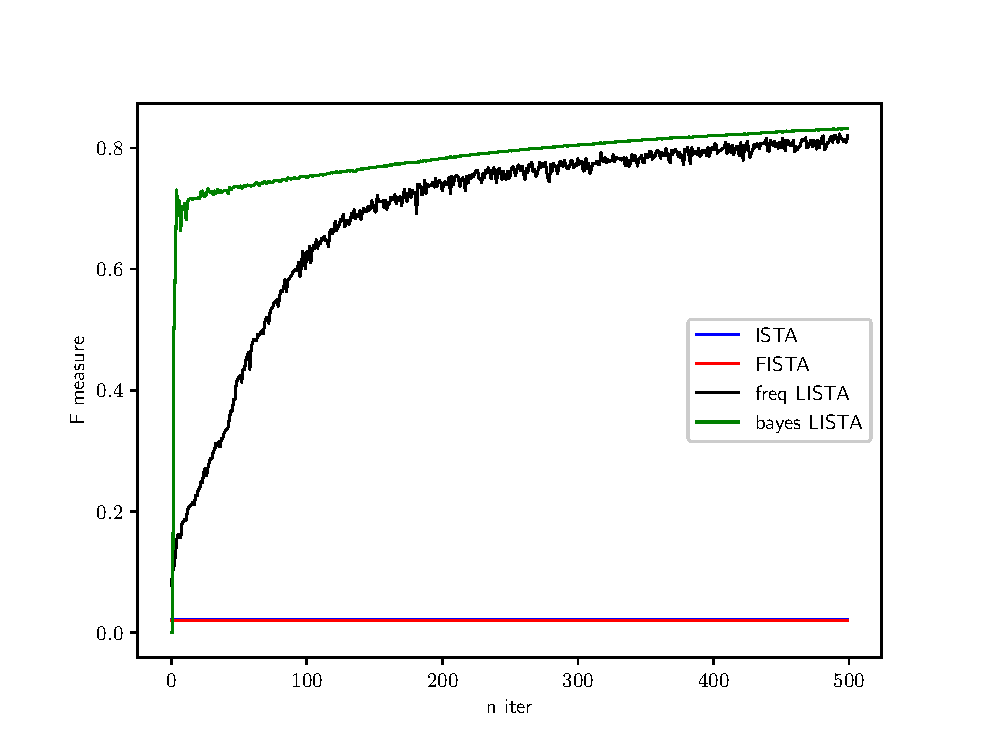
\includegraphics[width=0.5\columnwidth]{graphics/mnist/250_normalised_f_measure_train}}
%~
\subfloat[F measure for $K = 250$]{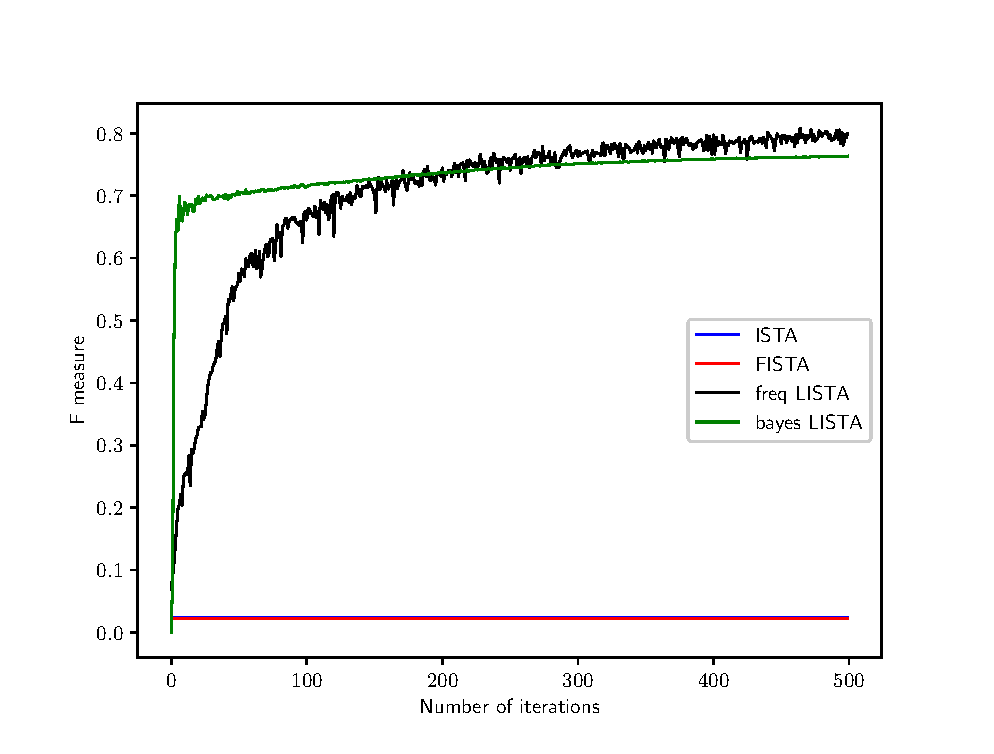
\includegraphics[width=0.4\columnwidth]{graphics/mnist/250_f_measure_valid}}
\caption{Predictive performance for different numbers of iterations on the \textsc{mnist} data with the observation size $K = 100$ (the top row) and $K = 250$ (the bottom row)}
\label{fig:mnist}
\end{figure}

\subsection{Active learning}
To demonstrate a potential scenario that can benefit from uncertainty estimates of the Bayesian \textsc{lista}, we consider the active learning example \cite{settles.tr09}. The active learning area researches ways to select new training subsets to reduce the total number of required supervision. One of the popular approaches in active learning is uncertainty sampling, when the data with the least certain predictions is chosen for labelling. We use a variance from Lemma~\ref{thm:moments_spsl} as a measure of uncertainty.

The data in this example is the \textsc{mnist} dataset with the observation size $K=100$. We use the training data of size $50$, the pool data of size $500$,  and the test data of size $100$. The algorithm learns on the training data for $50$ iterations and it is evaluated on the test data. To actively collect a next data point from the pool, the algorithm is used to predict a point with the highest uncertainty. The selected point is moved from the pool to the training data and the algorithm performs additional $10$ iterations on the updated training data. Overall, $10$ pool additions are performed. After every addition the performance is measured on the test data. We compare the actively updated approach of adding new points from the pool with the random approach that picks a new data point from the pool at random. The procedure is repeated for $20$ times with new randomly selected initial datasets.

Figure \ref{fig:active_learning_mnist} demonstrates performance of the active and non-active methods of updates with the Bayesian \textsc{lista}. The active approach with uncertainty sampling steadily demonstrates better results in terms of both quality measures. This means that the posterior distribution learnt by the Bayesian \textsc{lista} is an adequate estimate of the true posterior.
\begin{figure}[h]
\centering
\subfloat[\textsc{nmse}]{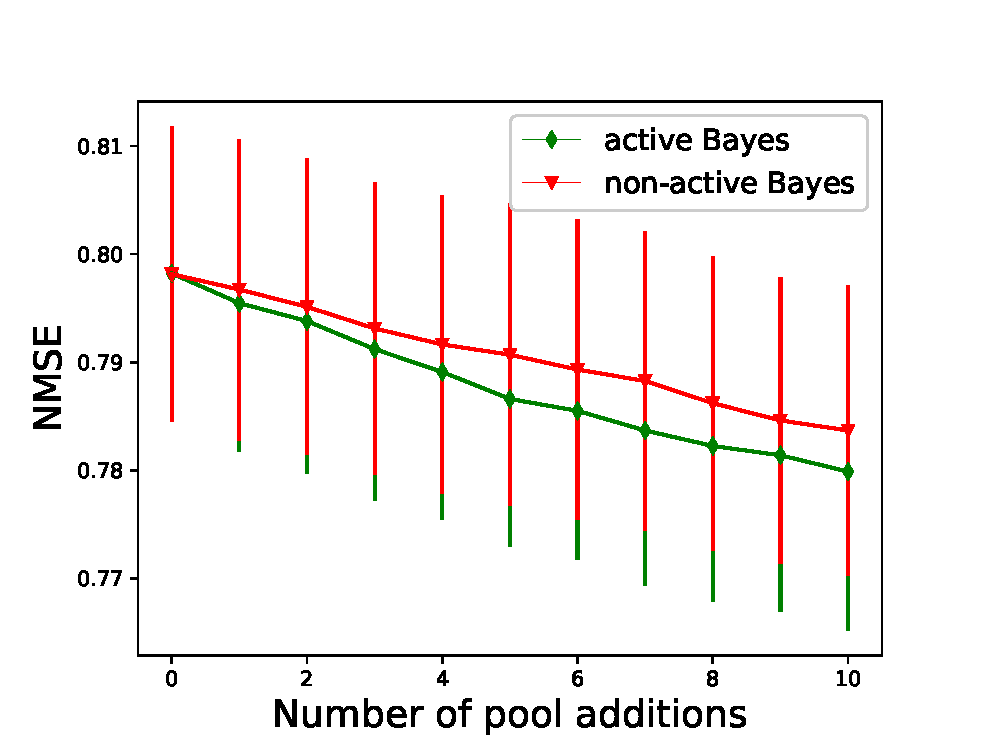
\includegraphics[width=0.4\columnwidth]{graphics/active_mnist/nmse_validation}}%
\subfloat[F measure]{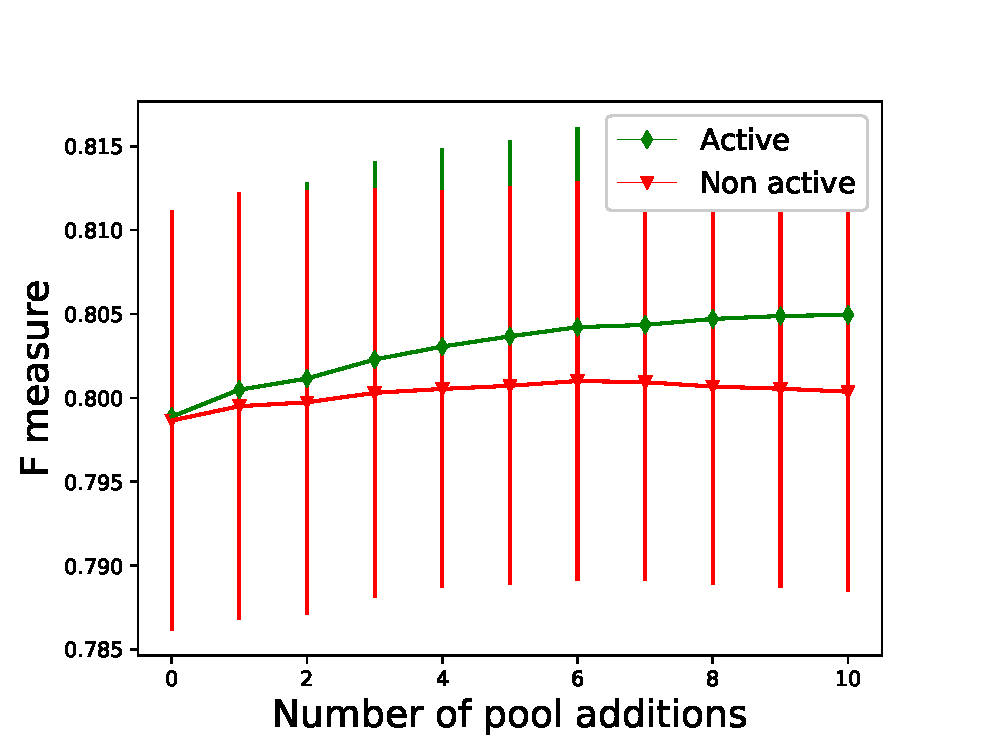
\includegraphics[width=0.4\columnwidth]{graphics/active_mnist/f_measure_validation}}
\caption{Performance for the active learning experiment on the \textsc{mnist} data. }
\label{fig:active_learning_mnist}
\end{figure}

\section{Conclusions and future work}
\label{sec:conclusions}
To the best of our knowledge, this is the first implementation of a Bayesian deep sparse coding algorithm. Although there are works on Bayesian sparsity in context of neural networks \cite{he2017bayesian}, they are not the Bayesian neural networks in the same sense as the Bayesian \textsc{lista} but rather the interpretation of the sparse Bayesian  learning algorithm as the long short-term memory network. We find not only correct predictions but also useful posterior estimates for the predictions.

We have presented the new method for propagating uncertainty through the soft thresholding function. %To achieve this goal
We have approximated the outputs of the function with a spike and slab distribution, and we have shown that this distribution can stay within the same family after linear transformation with Gaussian weights and inputs of a neural network. This allowed us to propose the Bayesian \textsc{lista} network and efficient inference algorithm that learns the distributions of the weights and makes the uncertainty estimates of the outputs. The forward propagation in the algorithm is based on the proposed uncertainty propagation method, the backward propagation is based on the probabilistic backpropagation method, that was remarkably expanded to account for multidimensionality of inputs and outputs, likelihood of the Bayesian \textsc{lista} and its recurrent nature.

Experiments on the synthetic and \textsc{mnist} datasets demonstrate that the proposed algorithm preserves the predictive accuracy of non-Bayesian methods while also providing posterior estimates. We also show that when the training data is very small the proposed algorithm significantly outperforms the classical \textsc{lista} in terms of predictive accuracy. Experiments on active learning demonstrate that the proposed Bayesian \textsc{lista} gives accurate posterior estimates that can be used for selection of a next data point where a label should be obtain at.

The shrinkage parameter $\lambda$ is currently treated as a deterministic hyperparameter for the Bayesian \textsc{lista}. In future we plan to incorporate it into the model treating it as a random variable. For this we will extend both the uncertainty propagation method to include uncertainty of $\lambda$ and the probabilistic backpropagation algorithm to estimate its posterior.

\small
\bibliography{bibliography}
\bibliographystyle{unsrtnat}

\end{document}
